\documentclass[11pt]{article}
\usepackage{neurips_2024}
\usepackage[utf8]{inputenc}
\usepackage[T1]{fontenc}
\usepackage{amsmath,amssymb}
\usepackage{graphicx}
\usepackage{booktabs}
\usepackage[pdfauthor={Abdullah Al Mahmud and Laila Sumiya Khan Nilo},
            pdftitle={Unsupervised Clustering of Hybrid Language Music Tracks Using Variational Autoencoders}]{hyperref}
\usepackage{float}
\usepackage{caption}
\usepackage{subcaption}
\usepackage{multirow}
\usepackage{xcolor}
\usepackage{natbib}

\title{Unsupervised Clustering of Hybrid Language Music Tracks\\Using Variational Autoencoders}

\author{
  Abdullah Al Mahmud \\
  Department of Computer Science and Engineering \\
  BRAC University \\
  \texttt{abdullah.al.mahmud@g.bracu.ac.bd}
  \And
  Laila Sumiya Khan Nilo \\
  Department of Computer Science and Engineering \\
  BRAC University \\
  \texttt{laila.sumiya.khan.nilo@g.bracu.ac.bd}
}

\date{}

\begin{document}
\maketitle

%% ============================================================
%% ABSTRACT
%% ============================================================
\begin{abstract}
Hybrid language music, particularly songs that combine Bangla and English lyrics, has become increasingly popular across digital streaming platforms. However, automatically organizing and understanding such music collections remains challenging due to linguistic diversity and variations in musical structure. In this paper, we propose an unsupervised learning framework for clustering hybrid language music tracks using a Variational Autoencoder (VAE). The VAE learns compact and meaningful representations by projecting high-dimensional audio features into a lower-dimensional latent space, where an encoder transforms the input into a latent distribution and a decoder reconstructs the original data. We extract latent representations from tabular audio features derived from the Million Song Dataset and perform clustering using K-Means. Our approach is evaluated against a PCA + K-Means baseline across six clustering quality metrics, including Silhouette Score, Calinski-Harabasz Index, Davies-Bouldin Index, Adjusted Rand Index, Normalized Mutual Information, and Cluster Purity. Experimental results demonstrate that VAE-learned representations yield substantially better cluster separation compared to linear dimensionality reduction, achieving a Silhouette Score of 0.211 versus 0.113 for PCA at the optimal configuration. We further analyze the effect of hyperparameters such as latent dimensionality and KL divergence weighting ($\beta$) on clustering quality and provide comprehensive visualizations of the learned latent space.
\end{abstract}

%% ============================================================
%% 1  INTRODUCTION
%% ============================================================
\section{Introduction}

Music has long transcended the boundaries of culture and geography, serving as a profound mode of human expression throughout history \citep{somyaji2025melody}. With the advent of artificial intelligence, the processes of music composition, arrangement, recording, and performance have undergone a substantial transformation \citep{fiorio2025clustering}. Hybrid language music, particularly songs that blend Bangla and English lyrics, has gained considerable popularity in modern music production. Amid the rapid expansion of online music platforms, efficient organization and analysis of large music collections has emerged as a significant challenge in music information retrieval (MIR).

A vast number of digital music tracks are generated and shared daily, and traditional approaches to organizing them rely on metadata such as artist names, genres, or manually assigned labels. However, hybrid compositions often blend diverse features including rhythm, melody, instrumentation, and language, making them difficult to categorize through conventional means. Classical clustering methods such as K-Means and Gaussian Mixture Models (GMMs), while widely applied, are limited to capturing local dependencies among data points and struggle with high-dimensional data \citep{mckinney2003features}, particularly in the presence of environmental noise in audio signals \citep{fiorio2025clustering}.

Deep generative models offer a promising alternative, as they are capable of processing high-dimensional data through unsupervised learning without reliance on labels. Among these, Variational Autoencoders (VAEs) \citep{kingma2014auto} and Generative Adversarial Networks (GANs) are the two most commonly adapted frameworks for unsupervised clustering. While both approaches perform clustering based on latent variables, VAEs possess a more structured latent space that directly benefits clustering \citep{fiorio2025clustering}, and they typically require smaller model architectures compared to GANs. VAEs have demonstrated considerable potential in generating meaningful and interpretable latent spaces \citep{carvalho2023exploring, wang2020pianotree}. A latent space provides a mathematical framework for manipulating and analyzing data using machine learning techniques and has been successfully adopted in applications such as music recommendation, style transfer, and music generation \citep{carvalho2023exploring}.

In this work, we explore a VAE-based representation learning approach for clustering hybrid language music tracks. The core idea is to extract compact latent representations of audio features and then apply clustering algorithms to group similar songs. Rather than manually defining rules to describe songs, the neural network learns patterns directly from the data. We apply this pipeline to a subset of the Million Song Dataset \citep{bertin2011million} containing 10,001 tracks, extracting 16 numeric audio features and learning compressed representations through VAE training. Our contributions are as follows:

\begin{itemize}
    \item We implement a VAE architecture for tabular music feature extraction and demonstrate its effectiveness for unsupervised clustering of hybrid language music tracks.
    \item We conduct a comprehensive hyperparameter sweep over latent dimensionality, KL divergence weight ($\beta$), and number of clusters.
    \item We compare VAE-based clustering against a PCA + K-Means baseline using six standard clustering metrics.
    \item We provide extensive visualizations including t-SNE and UMAP projections, reconstruction quality analysis, and ablation studies.
\end{itemize}

%% ============================================================
%% 2  RELATED WORK
%% ============================================================
\section{Related Work}

Variational Autoencoders were introduced by \citet{kingma2014auto} as a framework for learning latent variable models through amortized variational inference. The $\beta$-VAE variant \citep{higgins2017beta} subsequently introduced a tunable weight on the KL divergence term, enabling explicit control over the trade-off between reconstruction fidelity and latent space regularity. VAEs have demonstrated particular promise in the music domain, where they have been applied to generation, representation learning, and analysis tasks.

\citet{carvalho2023exploring} explored the latent spaces of tonal music using VAEs and showed that these spaces capture musically meaningful structure. Building on this direction, \citet{yang2019inspecting} proposed a method to inspect the pitch and rhythm interpretations of latent representations through disentanglement by augmentation. They examined the latent space learned by a compressed MusicVAE model and demonstrated that certain dimensions correspond to pitch change while others correspond to rhythm change, enabling modulation of average pitch and rhythm complexity independently. \citet{wang2020pianotree} introduced PianoTree VAE, a structured representation learning approach for polyphonic music that further illustrates the capacity of VAEs to capture hierarchical musical structure. In a related vein, \citet{somyaji2025melody} explored the use of VAEs for generating novel music by mixing styles, demonstrating the generative flexibility of VAE latent spaces across diverse musical traditions.

Beyond representation learning, clustering algorithms play a central role in unsupervised music analysis. \citet{araujo2025hybrid} presented a hybrid recommendation model that integrates K-Means clustering with a Multilayer Perceptron neural network to deliver coherent and diverse music recommendations. Their system achieved low track repetition (1.10\% overlap across 2,000 recommendations) while maintaining smooth transitions between tracks, confirming the utility of K-Means for grouping songs with similar characteristics. \citet{fiorio2025clustering} applied VAEs to the clustering of acoustic environments for hearing devices, demonstrating that VAE-based representations outperform classical approaches for clustering high-dimensional audio data.

In the broader machine learning literature, dimensionality reduction techniques including PCA, t-SNE \citep{van2008visualizing}, and UMAP \citep{mcinnes2018umap} are widely used for both preprocessing and visualization of high-dimensional features. The Million Song Dataset \citep{bertin2011million} has served as a standard benchmark for large-scale music analysis, and clustering methods such as K-Means, Gaussian Mixture Models, and spectral clustering have been extensively studied in the context of music organization \citep{mckinney2003features}. Our work builds on these foundations by combining VAE-based nonlinear dimensionality reduction with K-Means clustering and comparing the resulting representations against linear PCA baselines.

%% ============================================================
%% 3  METHOD
%% ============================================================
\section{Method}

Our pipeline consists of four stages: data preprocessing, VAE training for latent feature extraction, clustering on the learned latent space, and evaluation using both unsupervised and supervised metrics.

\subsection{Data Preprocessing}

We use a subset of the Million Song Dataset containing 10,001 tracks. From the available metadata, we select 16 numeric audio features: \textit{Duration}, \textit{KeySignature}, \textit{KeySignatureConfidence}, \textit{Tempo}, \textit{TimeSignature}, \textit{TimeSignatureConfidence}, \textit{Year}, \textit{ArtistFamiliarity}, \textit{Hotness}, \textit{end\_of\_fade\_in}, \textit{key}, \textit{keyConfidence}, \textit{Loudness}, \textit{mode}, \textit{mode\_confidence}, and \textit{start\_of\_fade\_out}. We exclude \textit{Danceability} and \textit{Energy} as they contain identical zero values across all tracks in this subset, and \textit{ArtistLatitude}/\textit{ArtistLongitude} due to 63\% missing values.

The \textit{Year} field uses 0 as a sentinel value for unknown release years (affecting 53.2\% of tracks); these are treated as missing and imputed with the median of known years. Remaining missing values are imputed using median imputation fitted on the training split. We apply Yeo-Johnson power transformation to reduce feature skewness, followed by winsorization at the 1st and 99th percentiles to mitigate the influence of extreme outliers. Finally, all features are standardized to zero mean and unit variance using statistics computed on the training set.

The data is split 90\%/10\% into training and validation sets. The scaler, imputer, and power transformer are fitted exclusively on the training data to prevent information leakage.

\subsection{VAE Architecture}

Our Variational Autoencoder consists of a symmetric encoder-decoder architecture. The encoder maps input features $\mathbf{x} \in \mathbb{R}^{16}$ through a series of fully connected hidden layers to produce parameters of the approximate posterior $q_\phi(\mathbf{z}|\mathbf{x}) = \mathcal{N}(\boldsymbol{\mu}_\phi(\mathbf{x}), \text{diag}(\boldsymbol{\sigma}^2_\phi(\mathbf{x})))$:

\begin{equation}
    \mathbf{h} = f_\phi(\mathbf{x}), \quad \boldsymbol{\mu} = W_\mu \mathbf{h} + b_\mu, \quad \log \boldsymbol{\sigma}^2 = W_\sigma \mathbf{h} + b_\sigma
\end{equation}

where $f_\phi$ denotes the encoder backbone consisting of two hidden layers with ReLU activations and dropout regularization ($p=0.1$). Latent samples are obtained via the reparameterization trick:

\begin{equation}
    \mathbf{z} = \boldsymbol{\mu} + \boldsymbol{\sigma} \odot \boldsymbol{\epsilon}, \quad \boldsymbol{\epsilon} \sim \mathcal{N}(\mathbf{0}, \mathbf{I})
\end{equation}

The decoder mirrors the encoder architecture and reconstructs the input as $\hat{\mathbf{x}} = g_\theta(\mathbf{z})$.

\subsection{Training Objective}

We train the VAE by maximizing the evidence lower bound (ELBO), which decomposes into a reconstruction term and a KL regularization term:

\begin{equation}
    \mathcal{L}(\theta, \phi; \mathbf{x}) = \underbrace{\mathbb{E}_{q_\phi(\mathbf{z}|\mathbf{x})}\left[\| \mathbf{x} - g_\theta(\mathbf{z}) \|^2 \right]}_{\text{Reconstruction (MSE)}} + \beta \cdot \underbrace{D_{\text{KL}}\left(q_\phi(\mathbf{z}|\mathbf{x}) \| p(\mathbf{z})\right)}_{\text{KL divergence}}
\end{equation}

where $p(\mathbf{z}) = \mathcal{N}(\mathbf{0}, \mathbf{I})$ is the standard Gaussian prior. The hyperparameter $\beta$ controls the trade-off between reconstruction fidelity and latent space regularity. To prevent posterior collapse during early training, we employ KL annealing: the effective KL weight is linearly increased from 0 to $\beta$ over the first 10 epochs.

The KL divergence for the diagonal Gaussian posterior admits a closed-form solution:

\begin{equation}
    D_{\text{KL}} = -\frac{1}{2} \sum_{j=1}^{d} \left(1 + \log \sigma_j^2 - \mu_j^2 - \sigma_j^2 \right)
\end{equation}

\subsection{Clustering}

After training, we extract the posterior mean $\boldsymbol{\mu}_\phi(\mathbf{x})$ for each track as its latent representation. Using the mean rather than sampling from the posterior provides deterministic, stable embeddings suitable for clustering. We apply K-Means clustering to these latent representations, sweeping the number of clusters $k$ from 2 to 15.

As a baseline, we apply PCA to reduce the original 16-dimensional feature space to the same dimensionality as the VAE latent space, followed by K-Means clustering with identical settings.

\subsection{Evaluation Metrics}

We evaluate clustering quality using three unsupervised metrics and three supervised metrics. The unsupervised metrics do not require ground-truth labels:

\textbf{Silhouette Score} measures how similar each point is to its own cluster relative to neighboring clusters:
\begin{equation}
    s(i) = \frac{b(i) - a(i)}{\max(a(i), b(i))}
\end{equation}
where $a(i)$ is the mean intra-cluster distance and $b(i)$ is the mean nearest-cluster distance. Values range from $-1$ to $1$; higher indicates better separation.

\textbf{Calinski-Harabasz Index} computes the ratio of between-cluster to within-cluster variance:
\begin{equation}
    \text{CH} = \frac{\text{tr}(B_k) / (k - 1)}{\text{tr}(W_k) / (n - k)}
\end{equation}
where $B_k$ and $W_k$ are the between- and within-cluster dispersion matrices. Higher values indicate better-defined clusters.

\textbf{Davies-Bouldin Index} measures the average similarity between each cluster and its most similar neighbor:
\begin{equation}
    \text{DB} = \frac{1}{k} \sum_{i=1}^{k} \max_{j \neq i} \frac{\sigma_i + \sigma_j}{d_{ij}}
\end{equation}
Lower values indicate better clustering, with zero being the theoretical optimum.

For supervised evaluation, we construct pseudo-ground-truth labels by binning tracks into six decade categories based on their release year: \textit{Unknown era} (Year = 0), \textit{Pre-1970s}, \textit{1970s}, \textit{1980s}, \textit{1990s}, and \textit{2000s+}. Using these labels, we compute:

\textbf{Adjusted Rand Index (ARI)} quantifies agreement between predicted clusters and true labels, adjusted for chance.

\textbf{Normalized Mutual Information (NMI)} measures the mutual information between cluster assignments and labels, normalized to $[0, 1]$:
\begin{equation}
    \text{NMI}(U, V) = \frac{2I(U; V)}{H(U) + H(V)}
\end{equation}

\textbf{Cluster Purity} computes the fraction of the dominant class within each cluster:
\begin{equation}
    \text{Purity} = \frac{1}{n} \sum_{k} \max_{j} |c_k \cap t_j|
\end{equation}

%% ============================================================
%% 4  EXPERIMENTS
%% ============================================================
\section{Experiments}

\subsection{Dataset}

Our experiments use a 10,001-track subset of the Million Song Dataset. The decade distribution is highly imbalanced: 53.2\% of tracks have unknown release years, while among dated tracks, 55.7\% are from the 2000s, 25.7\% from the 1990s, 9.4\% from the 1980s, 5.3\% from the 1970s, and 3.9\% from before 1970. This imbalance poses a notable challenge for supervised evaluation metrics, as the ``Unknown era'' category dominates the dataset.

\subsection{Implementation Details}

We implement the VAE in PyTorch. The encoder and decoder each consist of two hidden layers with 128 units, ReLU activations, and 10\% dropout. Training uses the Adam optimizer with a learning rate of $10^{-3}$ and batch size of 256 for 80 epochs. KL annealing is applied over the first 10 epochs.

\subsection{Hyperparameter Sweep}

To identify the optimal configuration, we conduct a grid search over three hyperparameters:

\begin{itemize}
    \item \textbf{Latent dimensionality}: $d \in \{8, 16, 32\}$
    \item \textbf{KL weight}: $\beta \in \{0.01, 0.05, 0.1, 0.5, 1.0\}$
    \item \textbf{Number of clusters}: $k \in \{2, 3, \ldots, 15\}$
\end{itemize}

Each configuration is evaluated across 5 random seeds (42--46) to assess stability. Clustering metrics are aggregated as mean $\pm$ standard deviation across seeds. The best configuration is selected by maximizing the mean Silhouette Score (for $k \geq 3$ to avoid trivially high scores from binary splits), with ties broken by the lowest Davies-Bouldin Index.

For the PCA baseline, we match the latent dimensionality and number of clusters to the VAE configuration, sweeping the same $k$ range. K-Means is initialized with 30 restarts (\texttt{n\_init=30}) for both methods to ensure convergence.

We additionally evaluate Gaussian Mixture Models (GMM) as an alternative to K-Means to assess whether the assumption of spherical clusters affects results.

%% ============================================================
%% 5  RESULTS
%% ============================================================
\section{Results}

\subsection{Best Configuration}

The hyperparameter sweep identifies $d = 8$, $\beta = 1.0$, $k = 8$ as the optimal configuration, achieving a mean Silhouette Score of 0.211 ($\pm$ 0.004) across 5 seeds. Table~\ref{tab:comparison} presents a comprehensive comparison between the VAE and PCA baselines at this configuration.

\begin{table}[H]
\centering
\caption{Clustering metrics comparison at the optimal configuration ($d=8$, $k=8$). Values are mean $\pm$ std over 5 seeds. Higher is better for all metrics except Davies-Bouldin.}
\label{tab:comparison}
\begin{tabular}{lccc}
\toprule
\textbf{Metric} & \textbf{VAE + K-Means} & \textbf{PCA + K-Means} & \textbf{Winner} \\
\midrule
Silhouette Score ($\uparrow$) & $\mathbf{0.211 \pm 0.004}$ & $0.113 \pm 0.002$ & VAE \\
Calinski-Harabasz ($\uparrow$) & $\mathbf{1916.3 \pm 28.2}$ & $950.9 \pm 5.1$ & VAE \\
Davies-Bouldin ($\downarrow$) & $\mathbf{1.262 \pm 0.021}$ & $1.832 \pm 0.008$ & VAE \\
\midrule
ARI ($\uparrow$) & $0.052 \pm 0.001$ & $0.052 \pm 0.001$ & Tie \\
NMI ($\uparrow$) & $\mathbf{0.135 \pm 0.003}$ & $0.118 \pm 0.006$ & VAE \\
Purity ($\uparrow$) & $\mathbf{0.593 \pm 0.001}$ & $0.590 \pm 0.002$ & VAE \\
\bottomrule
\end{tabular}
\end{table}

The VAE achieves substantially better cluster separation on all three unsupervised metrics: nearly double the Silhouette Score (0.211 vs.\ 0.113), more than double the Calinski-Harabasz Index (1916 vs.\ 951), and a 31\% lower Davies-Bouldin Index (1.26 vs.\ 1.83). On supervised metrics, the two methods perform similarly on ARI, while the VAE holds a modest advantage on NMI (0.135 vs.\ 0.118) and Purity (0.593 vs.\ 0.590). Figure~\ref{fig:comparison_bar} visualizes this comparison.

\begin{figure}[H]
\centering
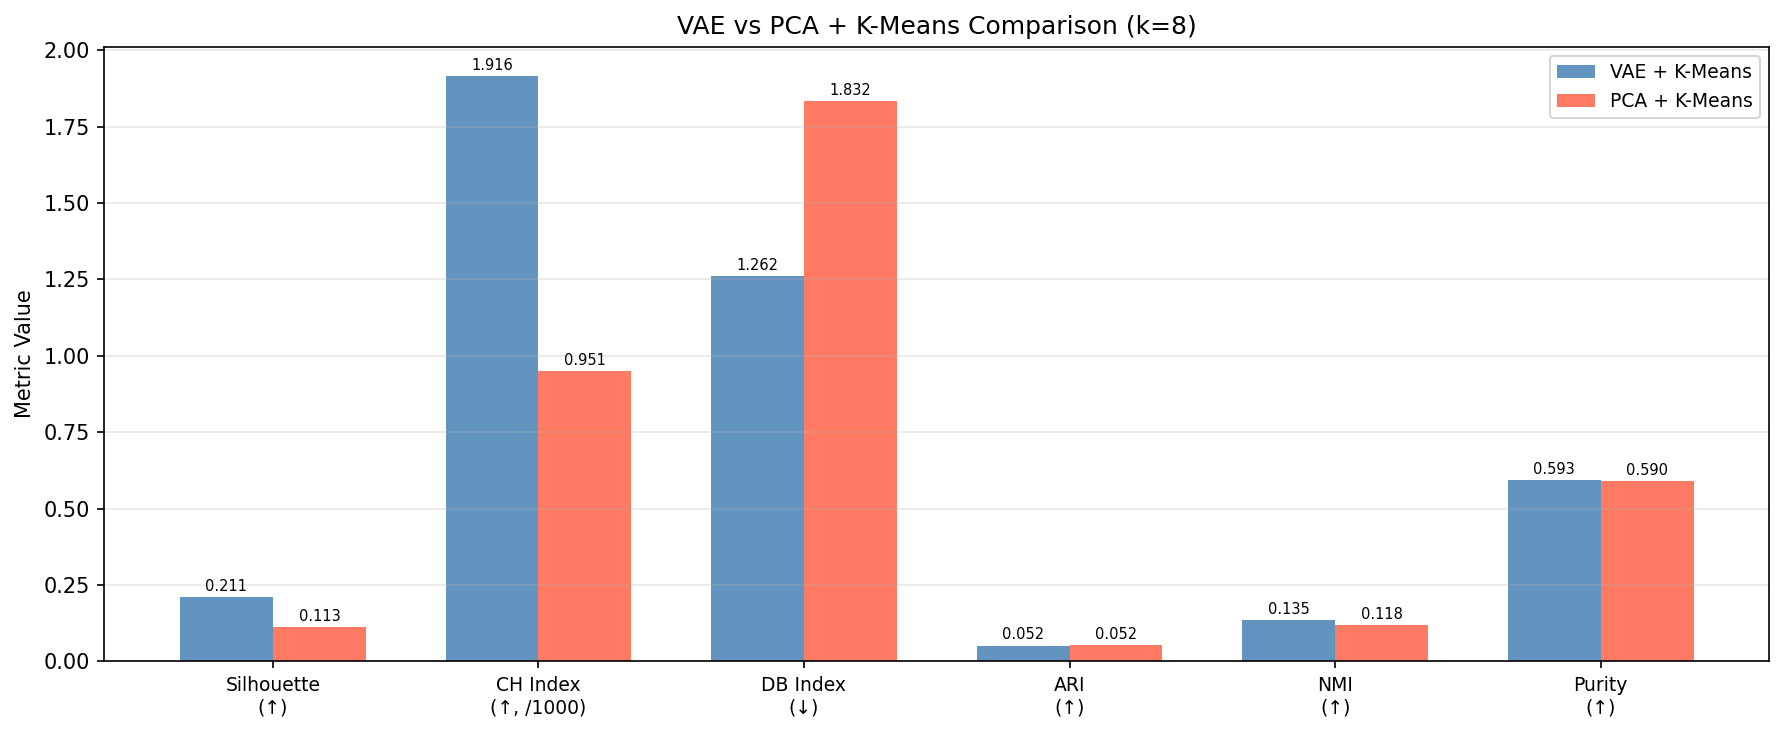
\includegraphics[width=\textwidth]{figures/comparison_bar.png}
\caption{Side-by-side comparison of VAE + K-Means vs.\ PCA + K-Means across all six metrics at $k = 8$. Calinski-Harabasz is scaled by $1/1000$ for readability.}
\label{fig:comparison_bar}
\end{figure}

\subsection{Training Dynamics}

Figure~\ref{fig:loss_curve} shows the training and validation loss curves for the best configuration. The model converges within approximately 20 epochs, with the initial rise corresponding to the KL annealing phase where the KL weight is linearly increased from 0 to $\beta = 1.0$ over 10 epochs. After annealing, both losses stabilize, indicating that the model achieves a good balance between reconstruction quality and latent space regularity without overfitting.

\begin{figure}[H]
\centering
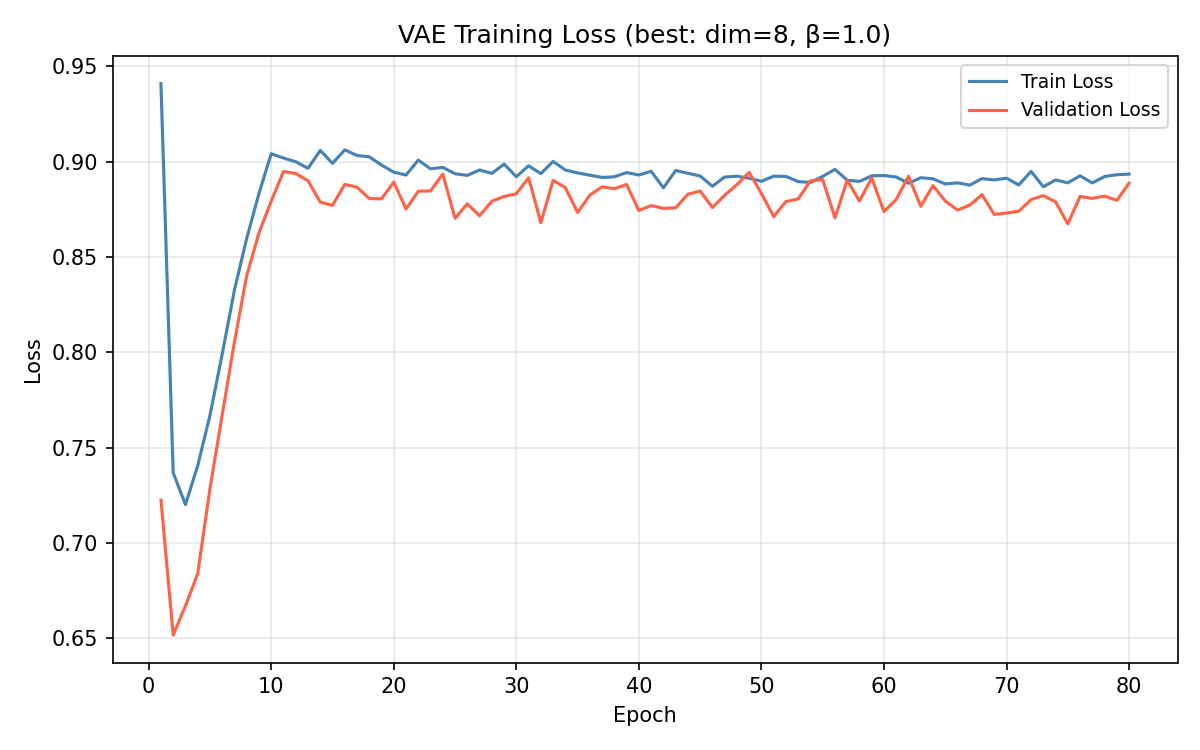
\includegraphics[width=0.75\textwidth]{figures/loss_curve_best.png}
\caption{Training and validation loss curves for the best VAE configuration ($d=8$, $\beta=1.0$). The initial rise reflects KL annealing over the first 10 epochs.}
\label{fig:loss_curve}
\end{figure}

\subsection{Clustering Quality Across $k$}

Figure~\ref{fig:metrics_vs_k} shows how unsupervised clustering metrics vary with the number of clusters for both VAE and PCA. The VAE consistently outperforms PCA across all tested values of $k$ on all three metrics. Notably, the performance gap is largest for moderate $k$ values (5--10), suggesting that the VAE latent space supports finer-grained cluster distinctions that PCA cannot capture.

\begin{figure}[H]
\centering
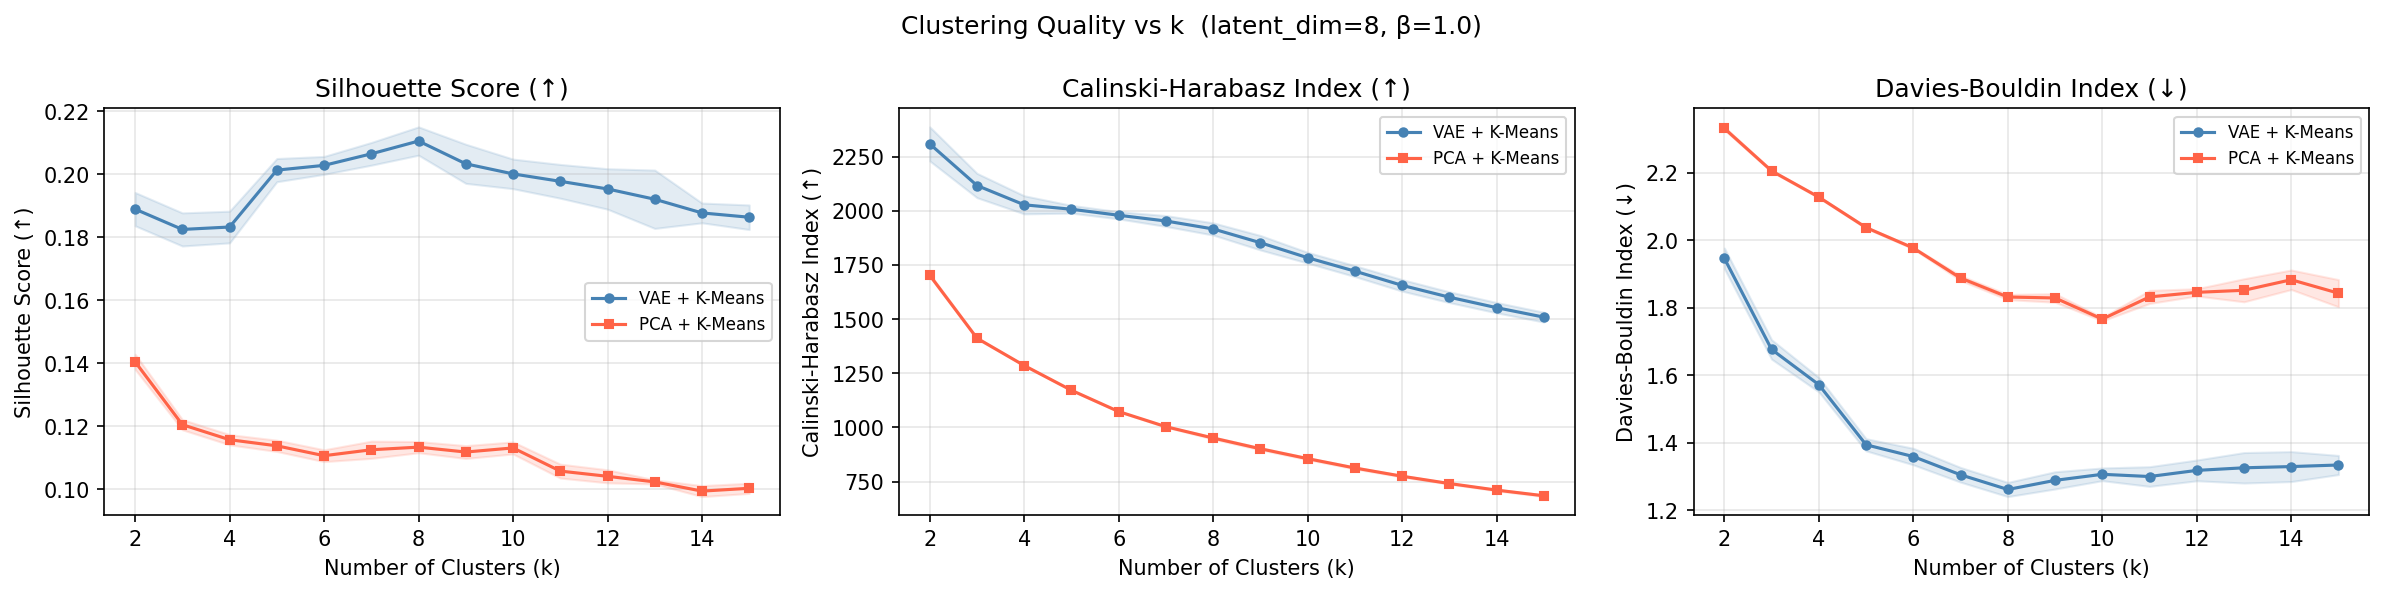
\includegraphics[width=\textwidth]{figures/metrics_vs_k.png}
\caption{Unsupervised clustering metrics vs.\ number of clusters $k$ for VAE + K-Means (blue) and PCA + K-Means (red). Shaded regions show $\pm 1$ standard deviation over 5 seeds. The VAE consistently achieves better Silhouette, Calinski-Harabasz, and Davies-Bouldin scores.}
\label{fig:metrics_vs_k}
\end{figure}

Figure~\ref{fig:supervised_vs_k} presents the supervised metrics across $k$. ARI and NMI generally increase with $k$ and plateau around $k = 6$--8, reflecting that finer granularity aligns better with the six decade categories used as pseudo-ground-truth labels. Purity is relatively stable across $k$ for both methods.

\begin{figure}[H]
\centering
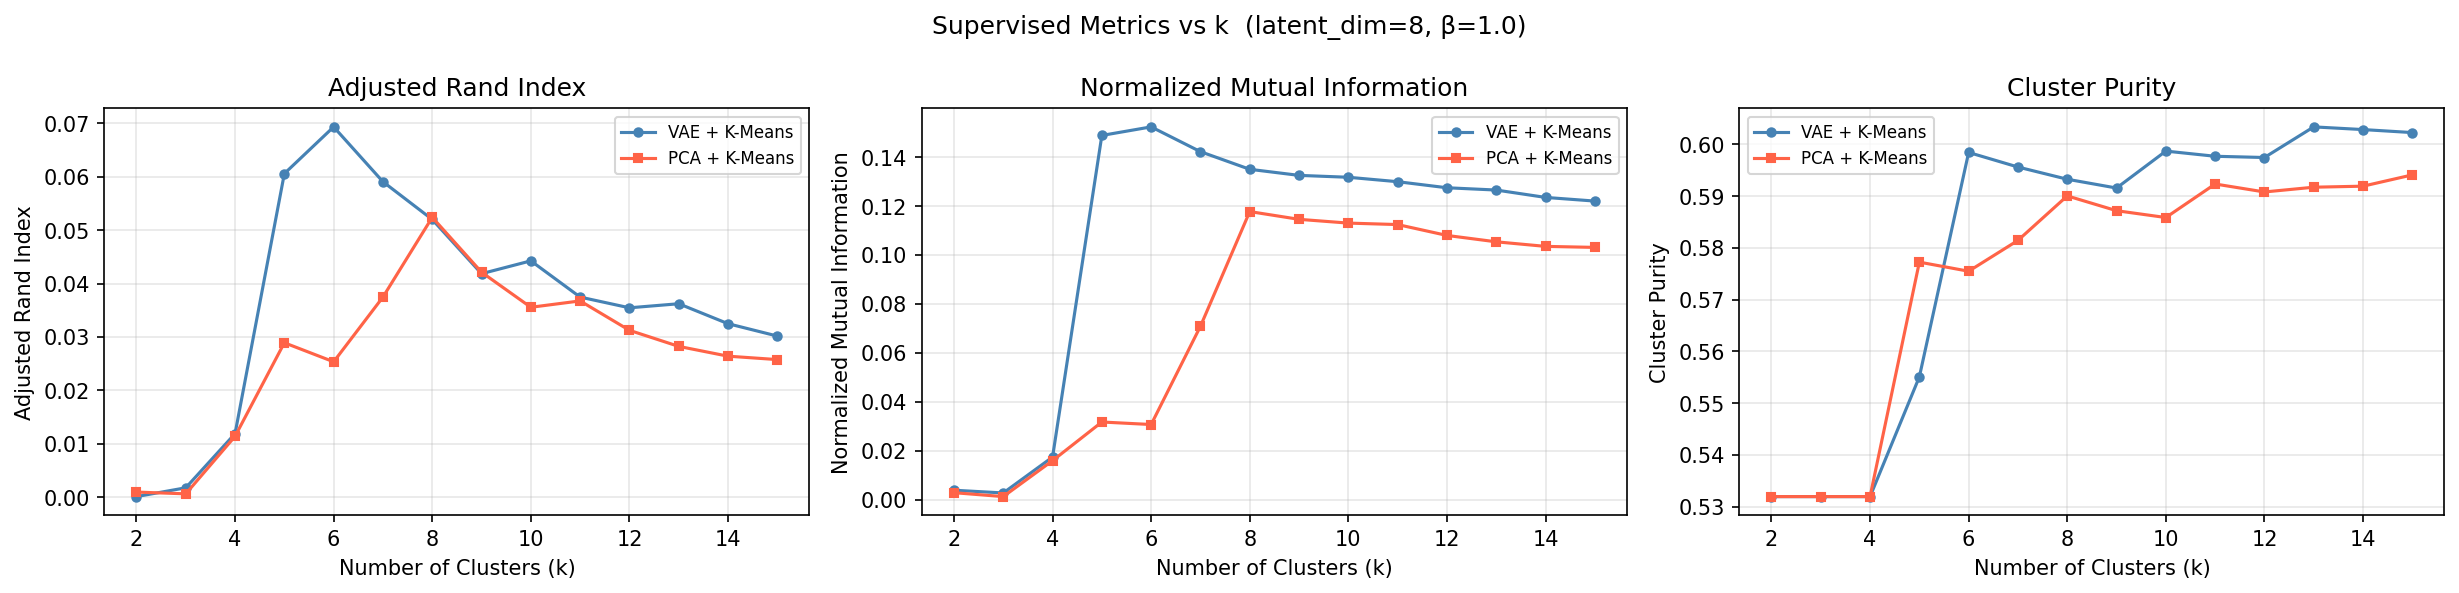
\includegraphics[width=\textwidth]{figures/supervised_metrics_vs_k.png}
\caption{Supervised clustering metrics (ARI, NMI, Purity) vs.\ $k$ for VAE and PCA methods. Both methods show similar supervised metric trends, with the VAE holding a slight edge on NMI.}
\label{fig:supervised_vs_k}
\end{figure}

\subsection{Effect of Hyperparameters}

\paragraph{Latent Dimensionality.} Smaller latent spaces produce better clustering. At $\beta = 1.0$ and $k = 8$, the Silhouette Score decreases from 0.211 ($d = 8$) to 0.110 ($d = 16$) to 0.089 ($d = 32$). This suggests that a lower-dimensional bottleneck forces the model to learn a more compressed and informative representation, while higher dimensions introduce redundancy that harms cluster separation.

\paragraph{KL Weight ($\beta$).} The KL weight has a pronounced effect on clustering quality. At $d = 8$ and $k = 8$, increasing $\beta$ from 0.01 to 1.0 improves the Silhouette Score from 0.101 to 0.211 and the Calinski-Harabasz Index from 824 to 1916 (Table~\ref{tab:beta_effect}). Lower $\beta$ values prioritize reconstruction at the expense of latent structure, resulting in an unregularized latent space that is less amenable to K-Means clustering. Conversely, $\beta = 1.0$ encourages a smoother, more Gaussian latent space where K-Means assumptions hold better.

\begin{table}[H]
\centering
\caption{Effect of $\beta$ on clustering quality at $d = 8$, $k = 8$.}
\label{tab:beta_effect}
\begin{tabular}{lccc}
\toprule
$\beta$ & Silhouette ($\uparrow$) & CH Index ($\uparrow$) & DB Index ($\downarrow$) \\
\midrule
0.01 & 0.101 & 824.0 & 1.935 \\
0.05 & 0.098 & 783.8 & 1.979 \\
0.10 & 0.097 & 759.1 & 1.968 \\
0.50 & 0.115 & 866.4 & 1.816 \\
1.00 & \textbf{0.211} & \textbf{1916.3} & \textbf{1.262} \\
\bottomrule
\end{tabular}
\end{table}

Figure~\ref{fig:beta_comparison} further illustrates this trend, showing a clear improvement across all metrics as $\beta$ increases.

\begin{figure}[H]
\centering
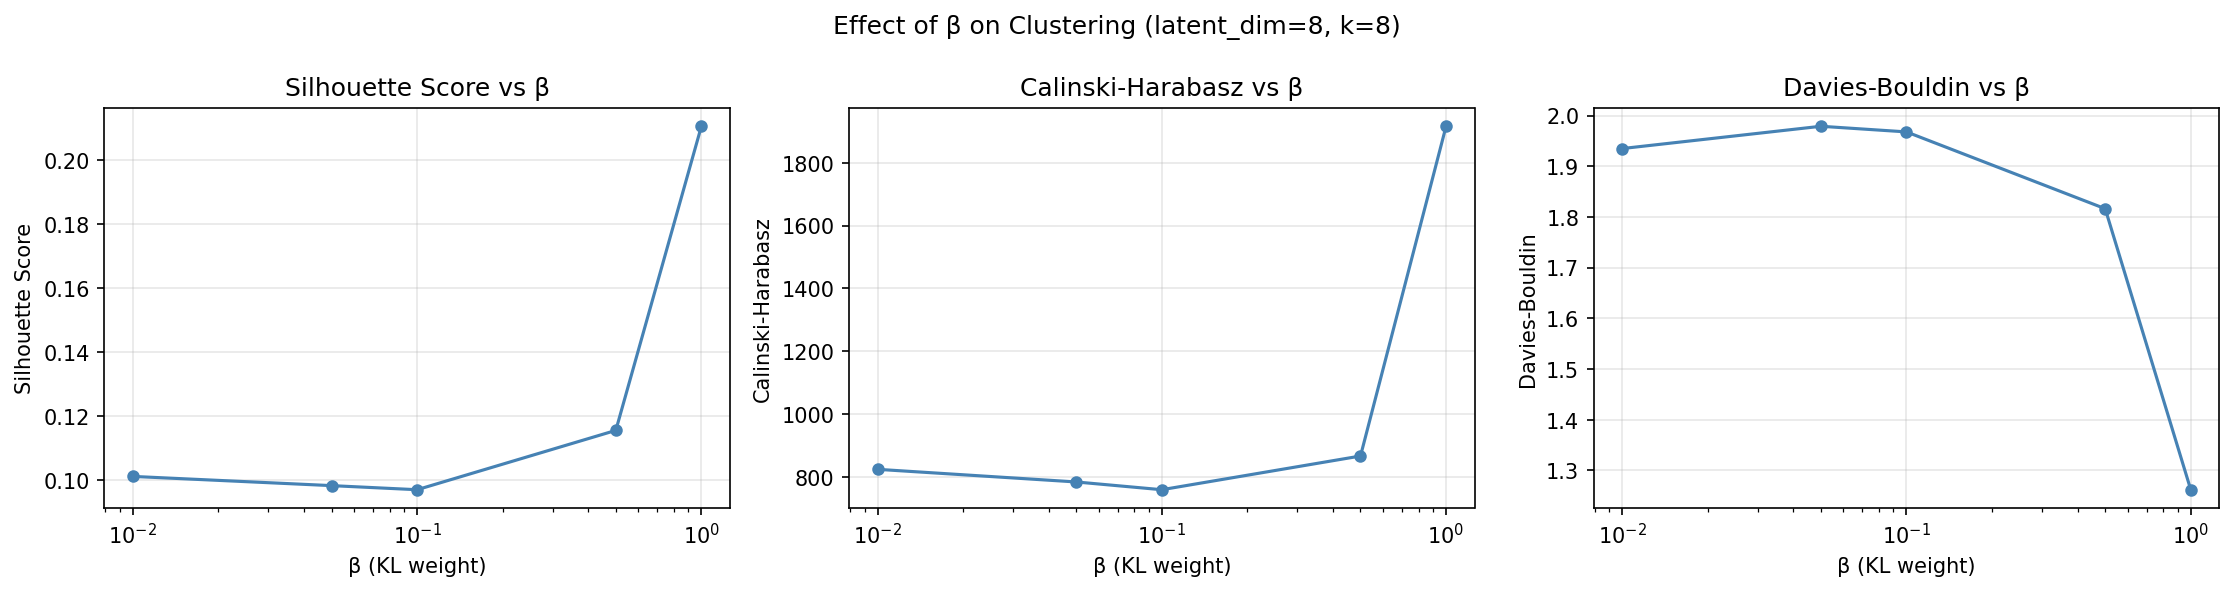
\includegraphics[width=\textwidth]{figures/beta_comparison.png}
\caption{Effect of $\beta$ on clustering metrics at $d = 8$, $k = 8$. Higher $\beta$ consistently improves all three unsupervised metrics.}
\label{fig:beta_comparison}
\end{figure}

\subsection{Latent Space Visualization}

Figure~\ref{fig:tsne_umap} presents t-SNE and UMAP projections of the VAE and PCA latent spaces, colored by K-Means cluster assignments. The VAE latent space exhibits more clearly separated cluster structures, particularly visible in the t-SNE projection where distinct groups are spatially separated. In contrast, the PCA latent space shows overlapping, less well-defined clusters.

\begin{figure}[H]
\centering
\begin{subfigure}[b]{0.48\textwidth}
    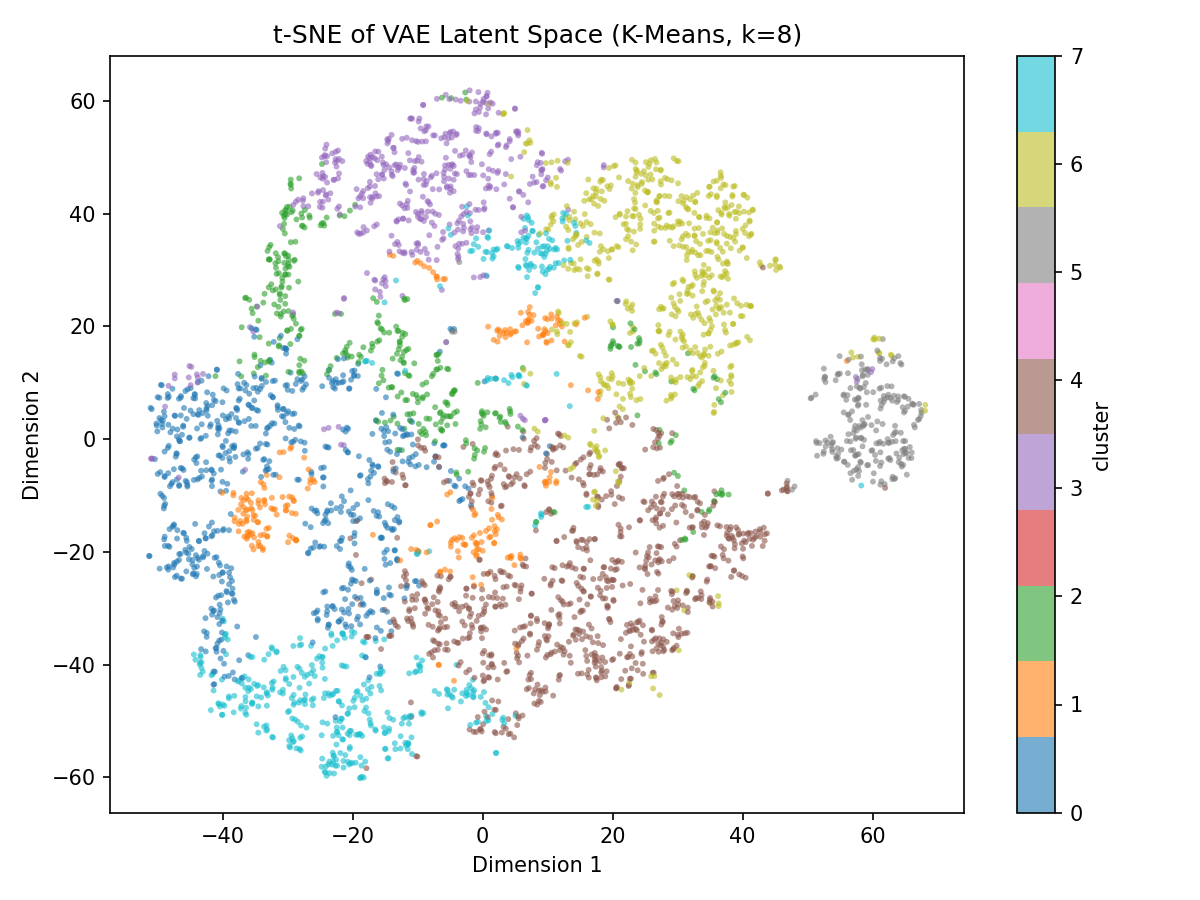
\includegraphics[width=\textwidth]{figures/tsne_vae_kmeans.png}
    \caption{t-SNE of VAE latent space}
\end{subfigure}
\hfill
\begin{subfigure}[b]{0.48\textwidth}
    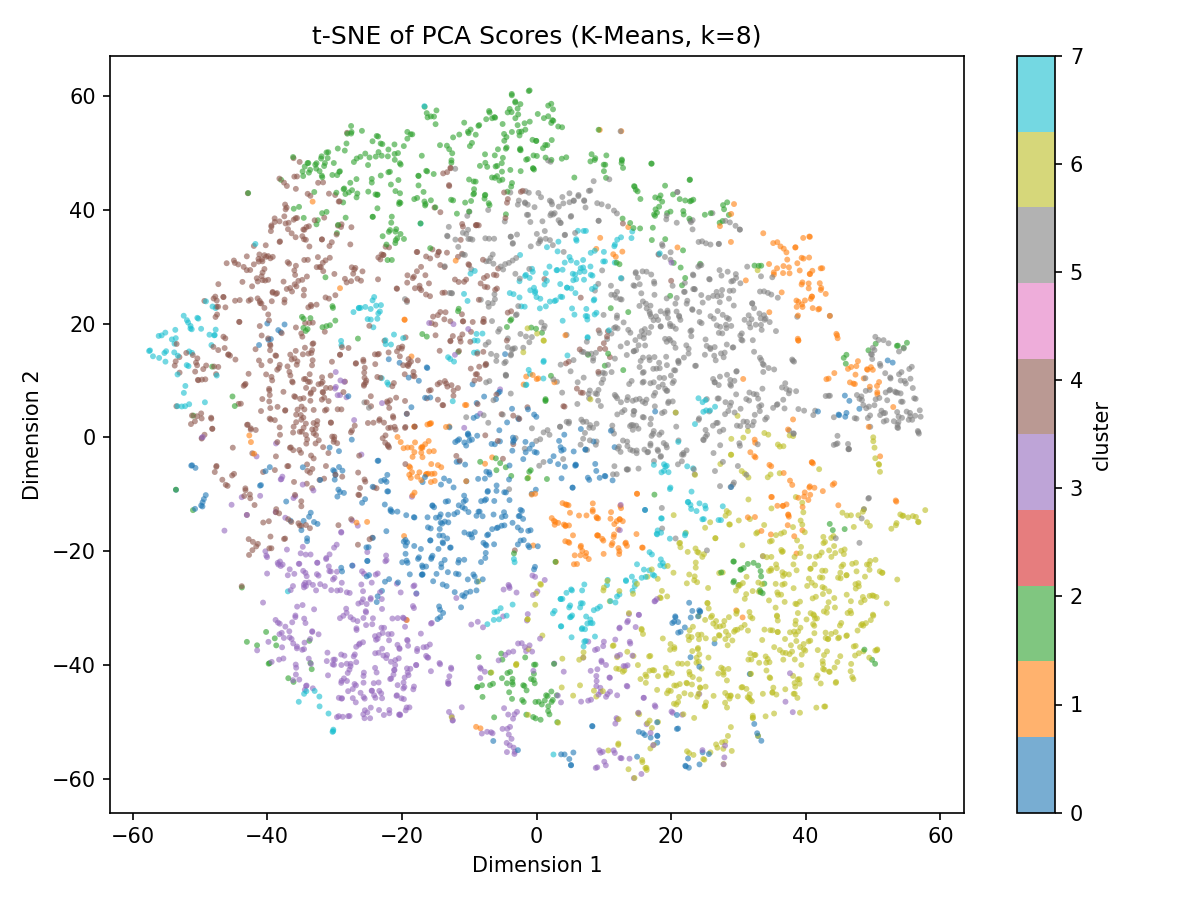
\includegraphics[width=\textwidth]{figures/tsne_pca_kmeans.png}
    \caption{t-SNE of PCA scores}
\end{subfigure}
\\[0.5em]
\begin{subfigure}[b]{0.48\textwidth}
    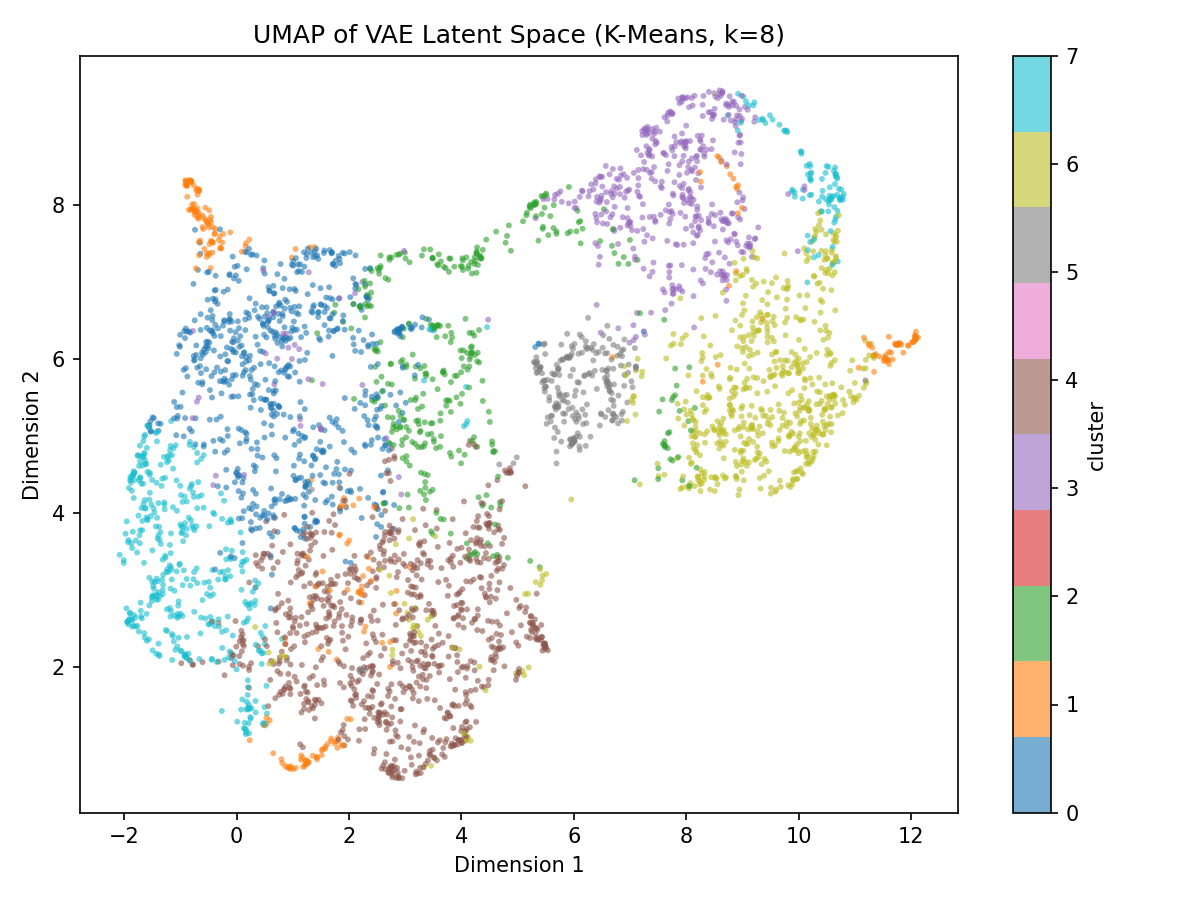
\includegraphics[width=\textwidth]{figures/umap_vae_kmeans.png}
    \caption{UMAP of VAE latent space}
\end{subfigure}
\hfill
\begin{subfigure}[b]{0.48\textwidth}
    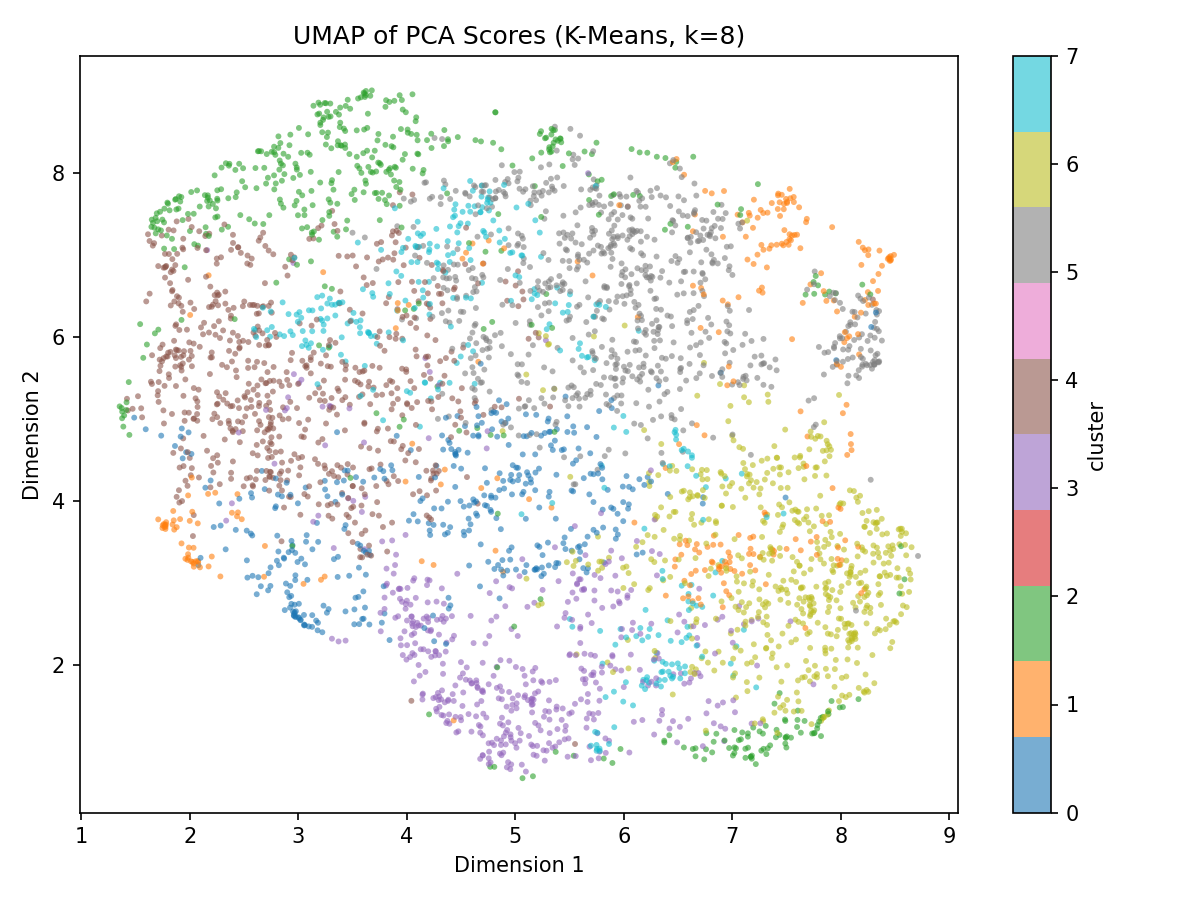
\includegraphics[width=\textwidth]{figures/umap_pca_kmeans.png}
    \caption{UMAP of PCA scores}
\end{subfigure}
\caption{2D projections of VAE (left) and PCA (right) latent spaces colored by K-Means cluster assignments ($k = 8$). The VAE latent space shows clearer cluster separation in both t-SNE and UMAP projections.}
\label{fig:tsne_umap}
\end{figure}

Figure~\ref{fig:decade_viz} shows the same t-SNE and UMAP projections colored by decade labels. The VAE latent space reveals partial temporal structure, with tracks from the 2000s and pre-1970s forming semi-distinct sub-regions. This suggests the VAE captures some temporal patterns in the audio features, though overlap remains substantial.

\begin{figure}[H]
\centering
\begin{subfigure}[b]{0.48\textwidth}
    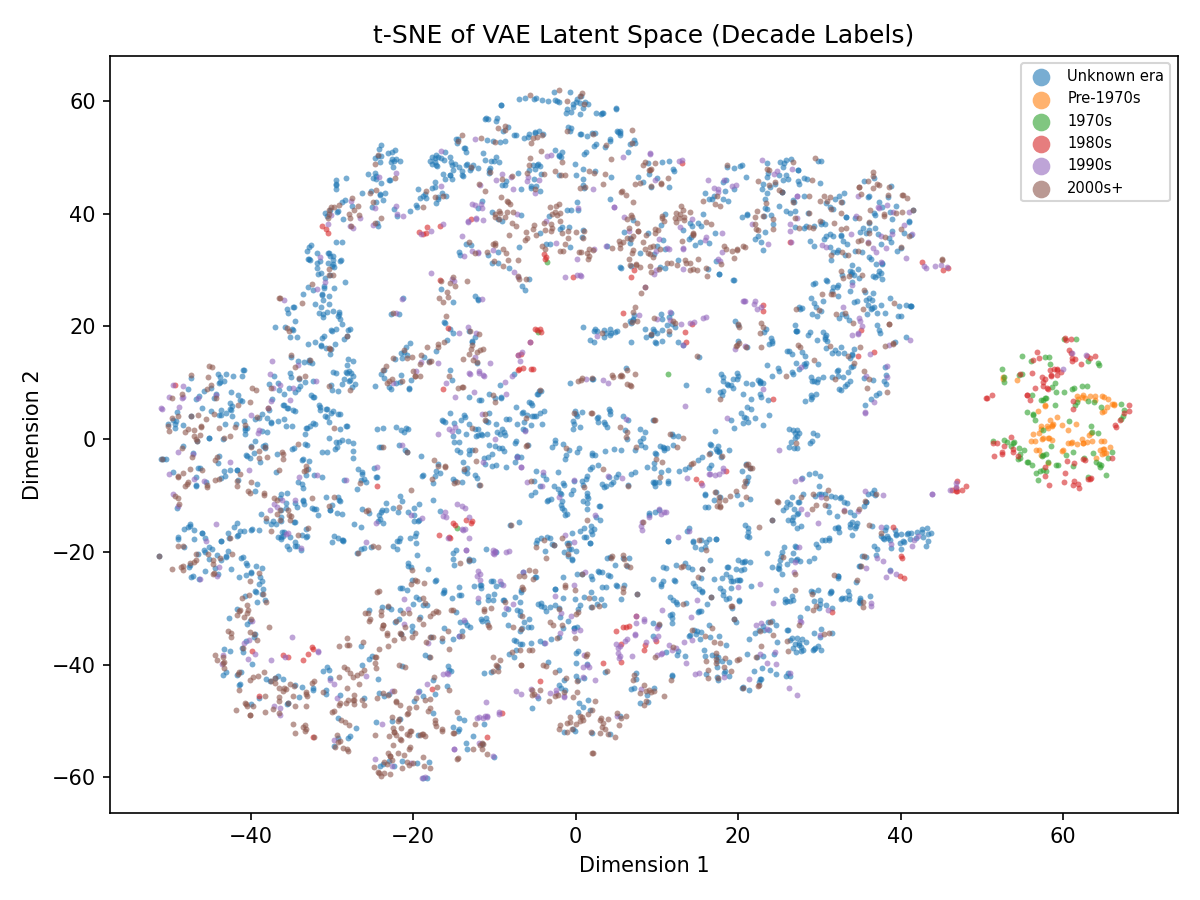
\includegraphics[width=\textwidth]{figures/tsne_vae_decades.png}
    \caption{t-SNE with decade labels}
\end{subfigure}
\hfill
\begin{subfigure}[b]{0.48\textwidth}
    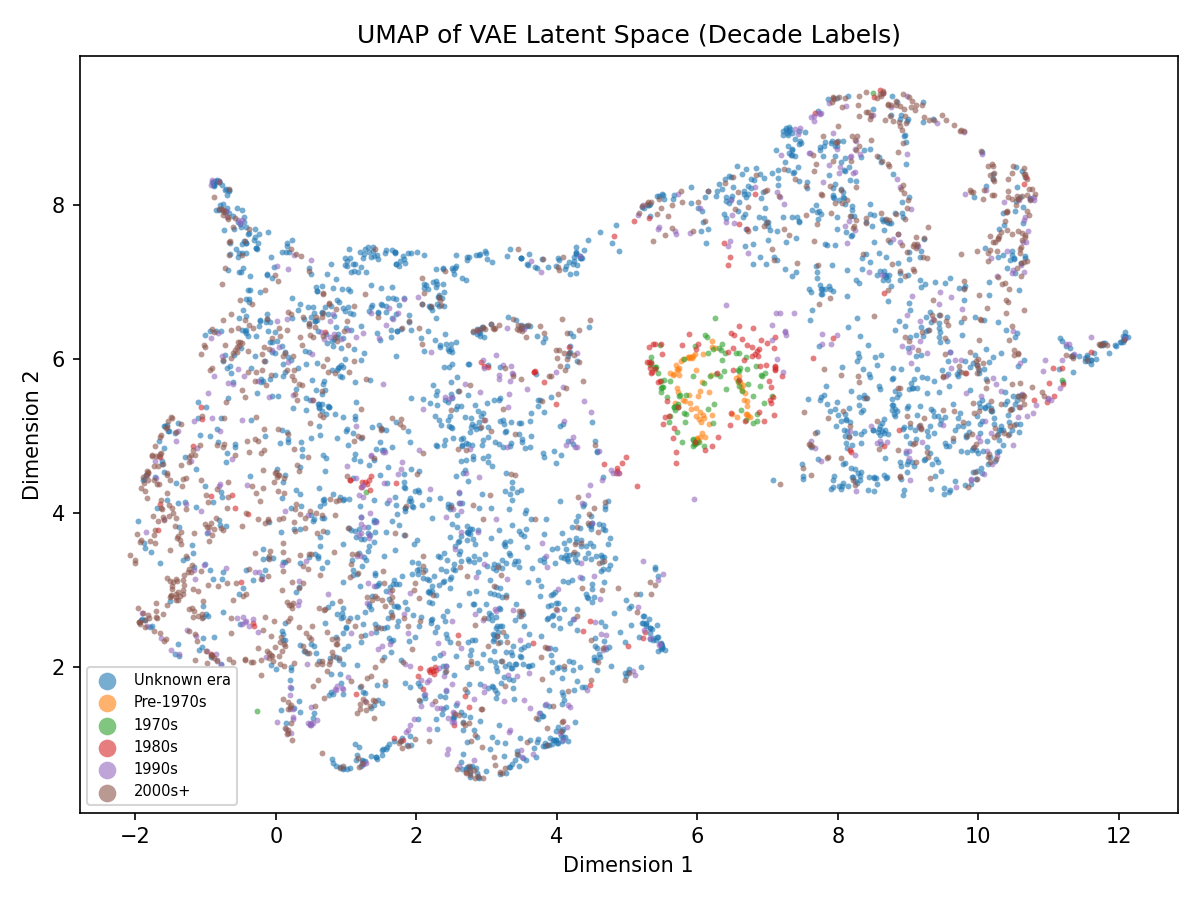
\includegraphics[width=\textwidth]{figures/umap_vae_decades.png}
    \caption{UMAP with decade labels}
\end{subfigure}
\caption{VAE latent space colored by decade-based pseudo-ground-truth labels. Some temporal clustering is visible, particularly for the 2000s+ and Pre-1970s groups.}
\label{fig:decade_viz}
\end{figure}

\subsection{Reconstruction Quality}

Figure~\ref{fig:recon_samples} shows the VAE's ability to reconstruct individual track features. The reconstruction broadly captures the feature profile of each track, with some features (e.g., \textit{Loudness}, \textit{Duration}) reconstructed more faithfully than others (e.g., \textit{mode}, \textit{KeySignature}). Figure~\ref{fig:recon_per_feature} provides a per-feature breakdown of mean absolute reconstruction error across 1,000 tracks. Continuous features such as \textit{Duration} and \textit{Loudness} exhibit lower reconstruction error, while discrete or binary features like \textit{mode} and \textit{KeySignature} are harder to reconstruct precisely.

\begin{figure}[H]
\centering
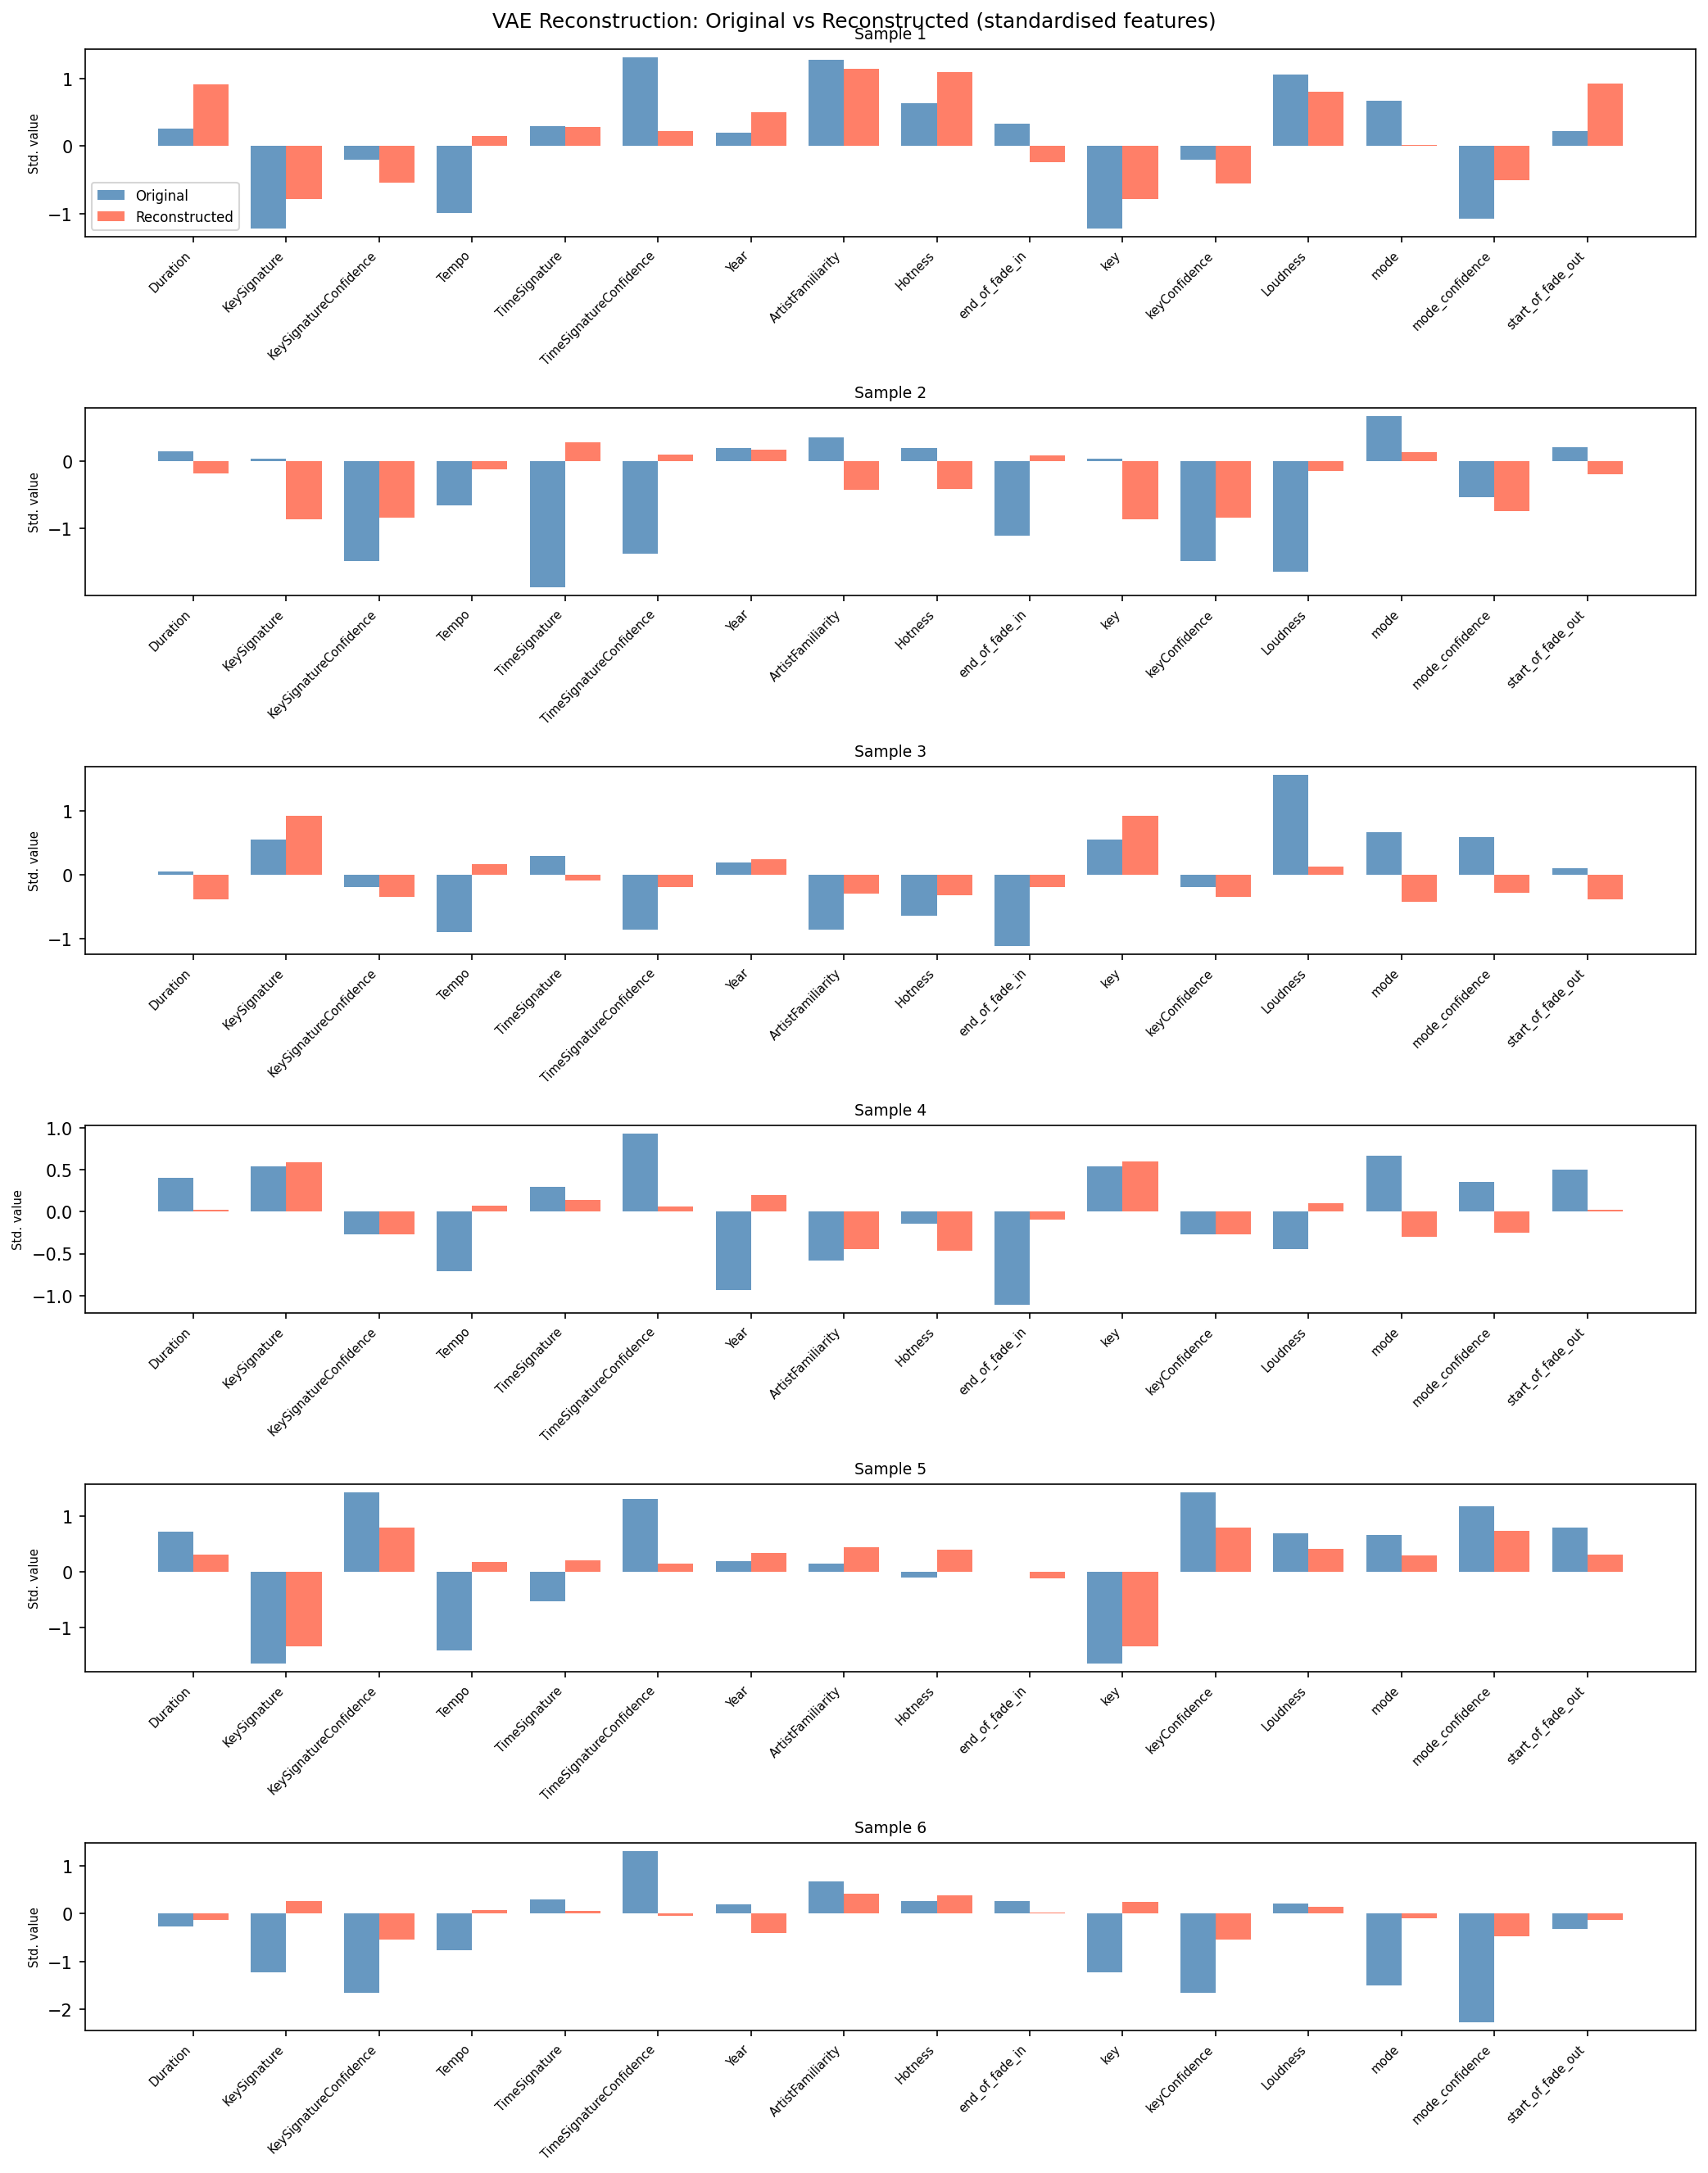
\includegraphics[width=\textwidth]{figures/reconstruction_samples.png}
\caption{Original vs.\ reconstructed features for six randomly sampled tracks. Blue bars are original (standardized) values; red bars are VAE reconstructions.}
\label{fig:recon_samples}
\end{figure}

\begin{figure}[H]
\centering
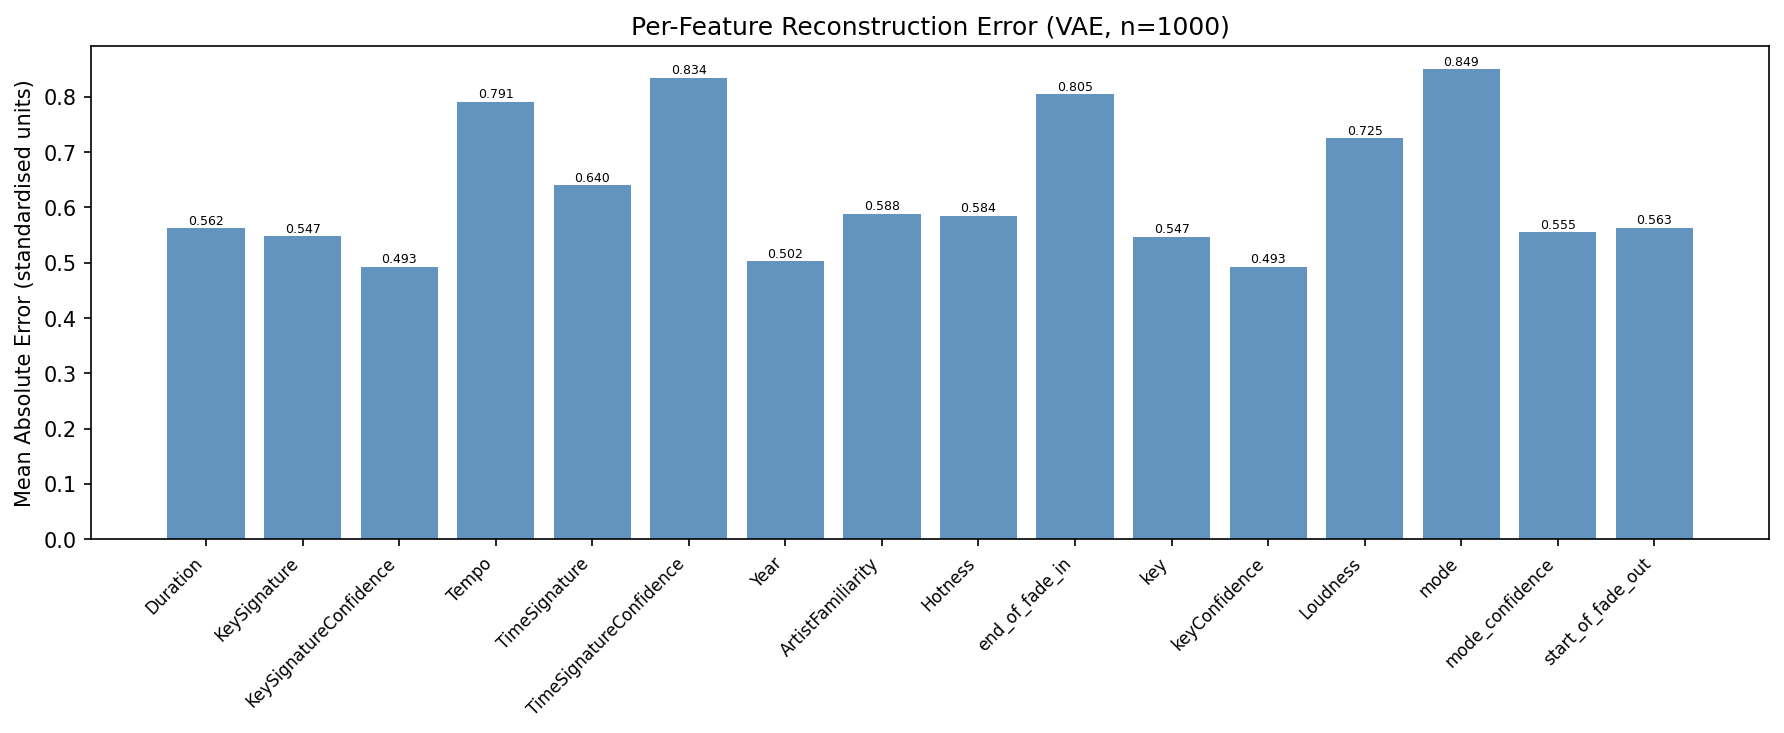
\includegraphics[width=0.85\textwidth]{figures/reconstruction_per_feature.png}
\caption{Mean absolute reconstruction error per feature across 1,000 tracks. Features with inherently discrete distributions (\textit{mode}, \textit{KeySignature}) are harder to reconstruct.}
\label{fig:recon_per_feature}
\end{figure}

\subsection{Latent Dimension Analysis}

Figure~\ref{fig:latent_dist} shows the distribution of values for each latent dimension. All eight dimensions are actively utilized, with varying spreads and shapes. Several dimensions exhibit bimodal or skewed distributions, suggesting they capture distinct modes of variation in the data. No dimension has collapsed to a near-zero constant, confirming the model avoids posterior collapse at $\beta = 1.0$ with KL annealing.

\begin{figure}[H]
\centering
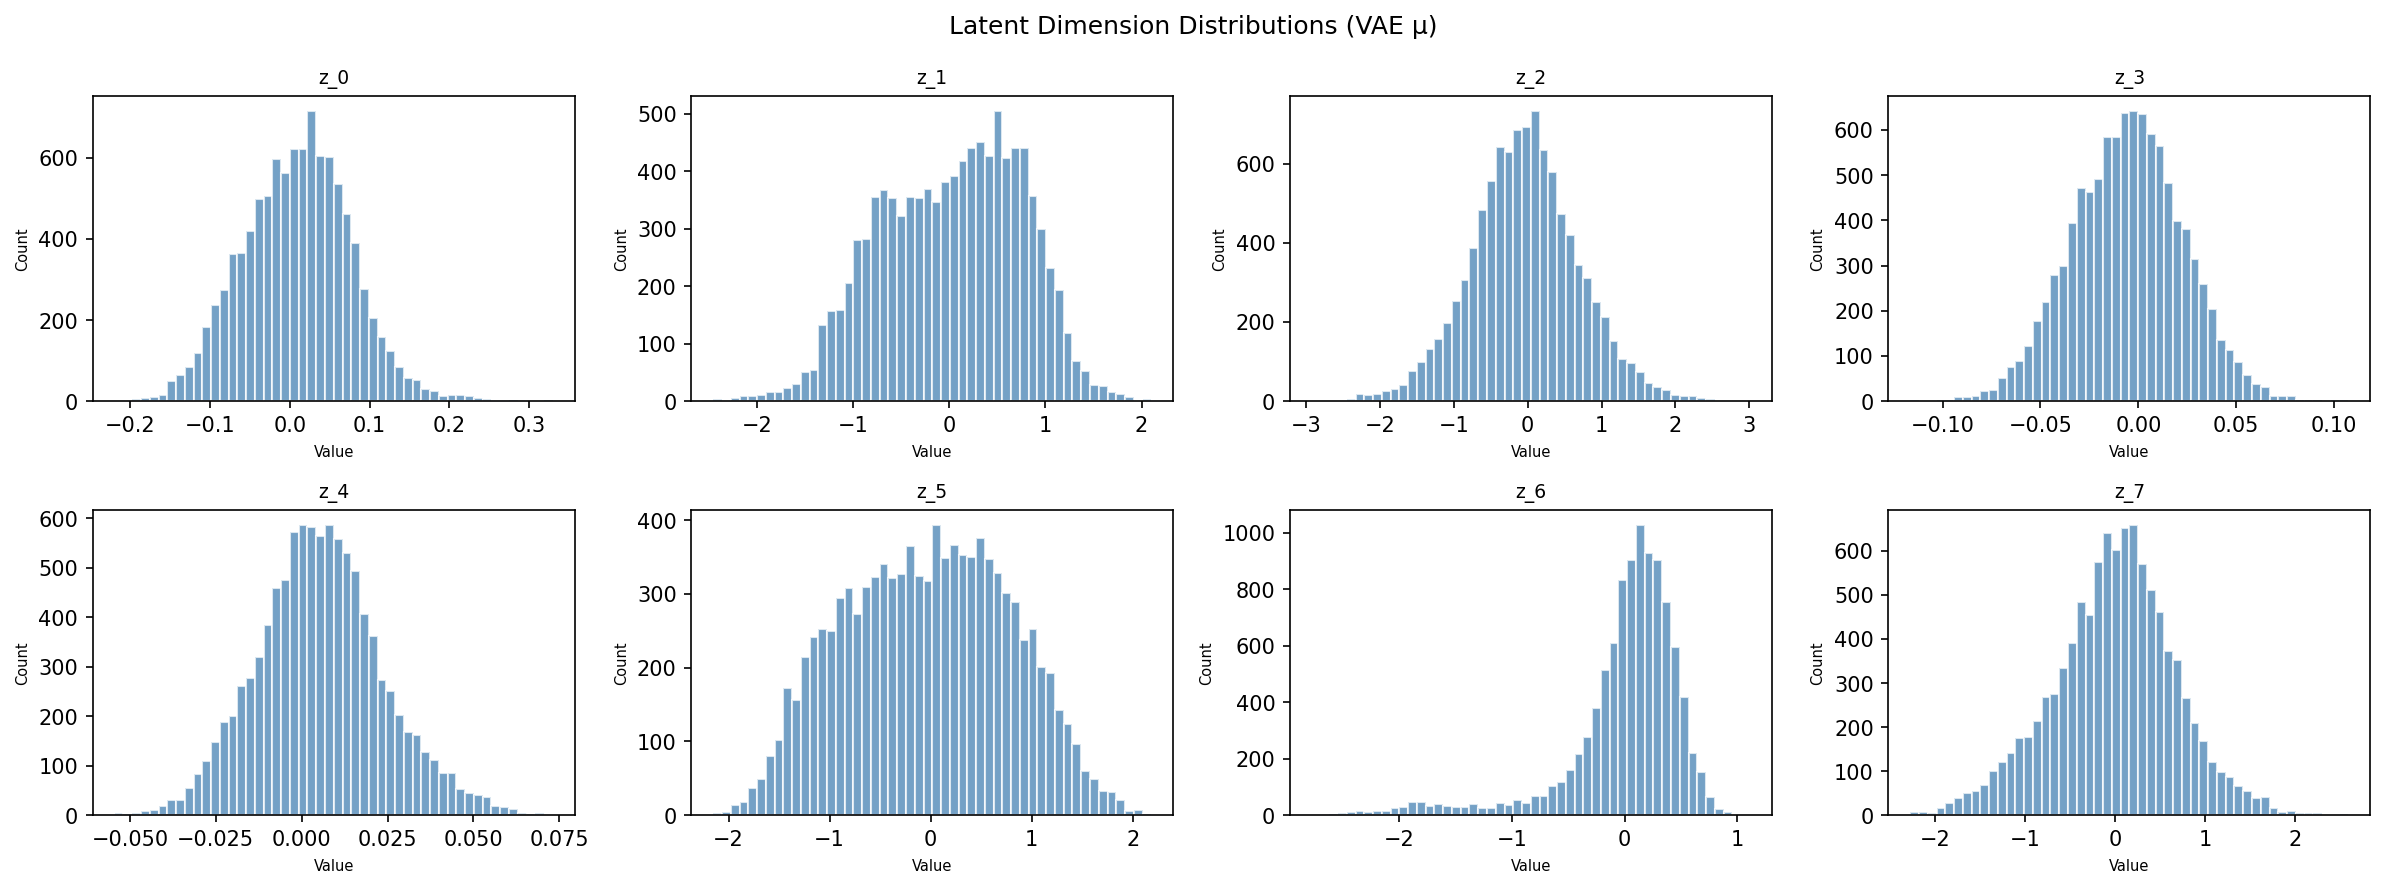
\includegraphics[width=0.85\textwidth]{figures/latent_distributions.png}
\caption{Distribution of latent dimension values ($\mu$) across all tracks. All dimensions are active, with some showing bimodal structure.}
\label{fig:latent_dist}
\end{figure}

\subsection{Cluster Selection Analysis}

Figure~\ref{fig:elbow} shows the elbow analysis for the VAE-based clustering. The Silhouette Score decreases gradually as $k$ increases beyond 5, while the Calinski-Harabasz Index decreases and the Davies-Bouldin Index remains relatively stable. The optimal $k = 8$ represents a good balance between granularity and separation quality.

\begin{figure}[H]
\centering
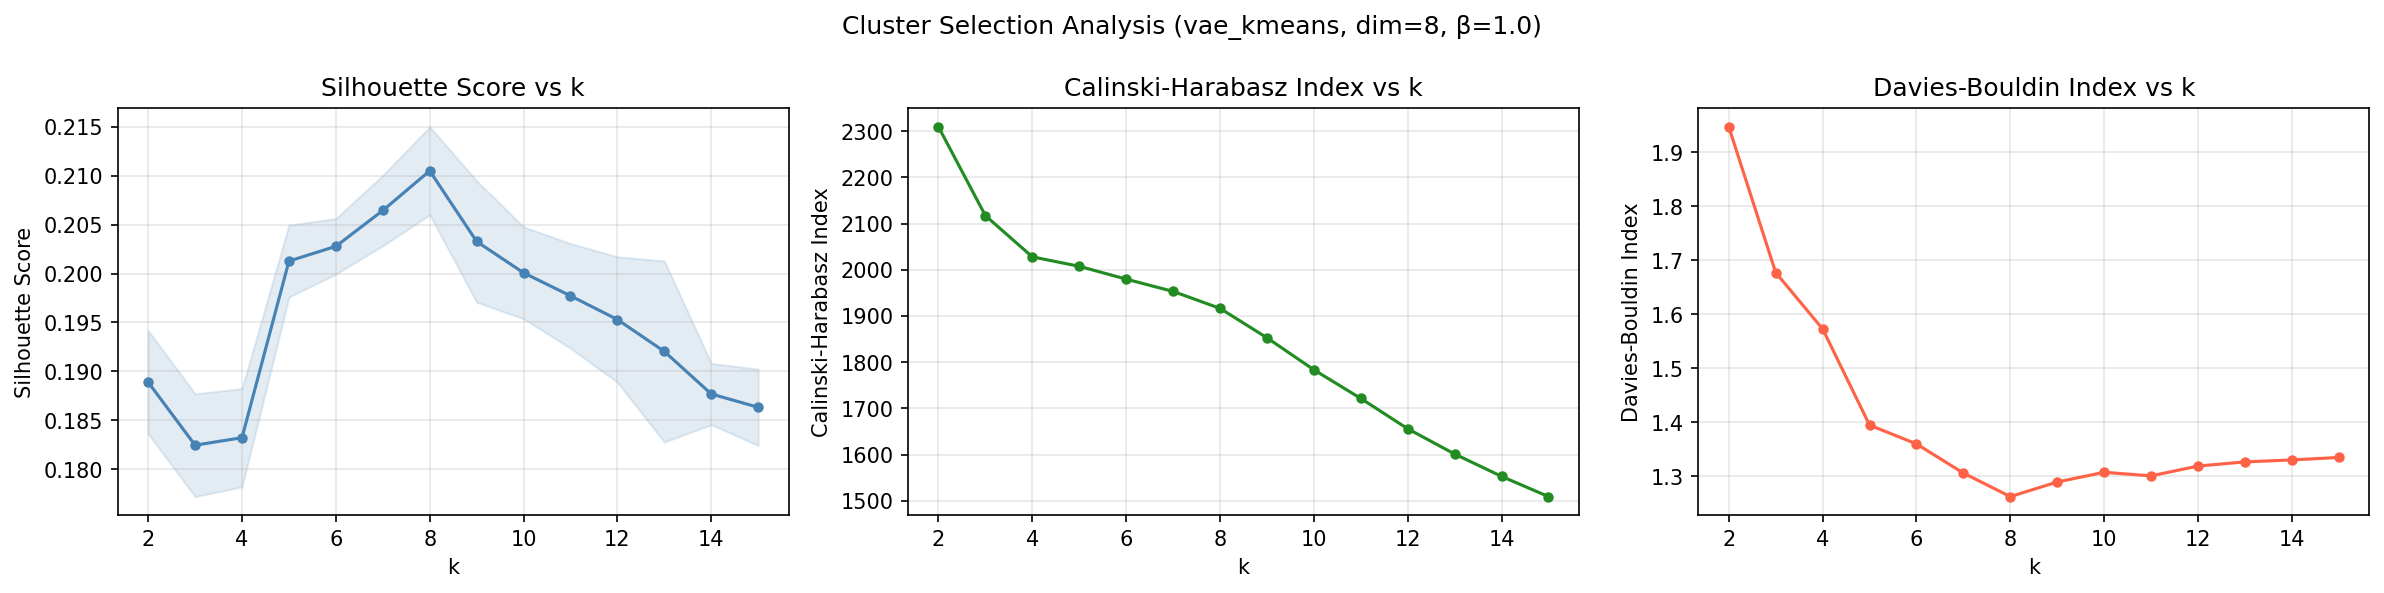
\includegraphics[width=\textwidth]{figures/elbow_vae.png}
\caption{Cluster selection analysis for VAE + K-Means ($d = 8$, $\beta = 1.0$). The Silhouette Score peaks at lower $k$ but $k = 8$ provides a good balance across all metrics.}
\label{fig:elbow}
\end{figure}

%% ============================================================
%% 6  DISCUSSION
%% ============================================================
\section{Discussion}

\subsection{VAE Superiority on Unsupervised Metrics}

The most notable finding is the substantial advantage of the VAE over PCA on unsupervised clustering metrics. The VAE achieves a Silhouette Score of 0.211, nearly double that of PCA (0.113), and comparable gaps are observed in the Calinski-Harabasz and Davies-Bouldin indices. This advantage arises from the VAE's capacity to learn nonlinear transformations that reshape the feature space into one where isotropic Gaussian assumptions---which K-Means implicitly relies upon---hold more naturally. PCA, as a linear method, can only rotate and scale the feature space, leaving nonlinear structures unresolved.

The observation that $\beta = 1.0$ yields the best clustering further supports this interpretation. The KL divergence term at unit weight encourages the latent space to approximate an isotropic Gaussian prior, which directly aligns with the spherical cluster assumption underlying K-Means. Lower $\beta$ values prioritize reconstruction fidelity at the expense of latent structure, confirming a fundamental trade-off between generative quality and clustering utility.

\subsection{Supervised Metric Analysis}

Despite strong performance on unsupervised metrics, supervised metrics remain modest (ARI $\approx$ 0.05, NMI $\approx$ 0.14). This outcome is largely attributable to the nature of our pseudo-ground-truth labels. Decade-based labels serve as a coarse proxy for musical similarity: tracks from the same decade can be stylistically diverse, while tracks from different decades may share similar audio characteristics. Furthermore, the ``Unknown era'' category (53.2\% of tracks) functions as a catch-all group that inflates purity while providing no meaningful semantic information.

These results underscore a fundamental limitation of evaluating unsupervised methods using weak proxies for ground truth. The clusters discovered by the VAE may capture acoustically meaningful patterns (e.g., loudness trends, tempo preferences, production styles) that do not align neatly with decade boundaries. A more musically informative label set---such as genre annotations---would likely yield higher supervised scores.

\subsection{Latent Dimensionality}

The finding that $d = 8$ outperforms $d = 16$ and $d = 32$ is noteworthy, given that the input space comprises 16 dimensions. A latent space smaller than the input imposes a genuine information bottleneck, compelling the model to retain only the most salient factors of variation. In contrast, $d = 32$ provides greater capacity than the input itself, which allows the model to learn a near-identity mapping that offers little advantage over the raw features.

\subsection{Limitations}

Several limitations of this work should be acknowledged. First, our features consist exclusively of tabular metadata from the Million Song Dataset; incorporating raw audio features (e.g., MFCCs, spectrograms) or textual lyrics could yield richer representations. Second, the substantial class imbalance in the dataset---more than half the tracks lack release year information---limits the utility of decade-based evaluation. Third, our VAE architecture is relatively simple; more sophisticated designs such as conditional VAEs or hierarchical VAEs could potentially capture additional structure in the data.

%% ============================================================
%% 7  CONCLUSION
%% ============================================================
\section{Conclusion}

In this paper, we presented a VAE-based unsupervised pipeline for clustering hybrid language music tracks using tabular audio features from the Million Song Dataset. Through a comprehensive hyperparameter sweep over latent dimensionality, KL divergence weight, and number of clusters---evaluated across five random seeds---we demonstrated that VAE-learned representations yield substantially better cluster separation than PCA baselines across all unsupervised metrics.

The optimal configuration ($d = 8$, $\beta = 1.0$, $k = 8$) achieves a Silhouette Score of 0.211, nearly doubling the PCA baseline of 0.113, while the Calinski-Harabasz Index improves by over 100\% and the Davies-Bouldin Index decreases by 31\%. Our analysis reveals that stronger KL regularization and lower latent dimensionality are essential to producing cluster-friendly representations, as they encourage a smooth, compact latent space that aligns well with the assumptions underlying K-Means clustering.

Several directions for future work merit exploration. Incorporating multi-modal features such as audio spectrograms and lyrics embeddings could enrich the learned representations. More expressive VAE variants, including $\beta$-VAE with disentanglement objectives and conditional VAEs, may capture additional structure in the data. Finally, alternative clustering methods such as spectral clustering and DBSCAN could be investigated to further improve both unsupervised and supervised clustering quality.

%% ============================================================
%% REFERENCES
%% ============================================================
\bibliographystyle{plainnat}

\begin{thebibliography}{13}

\bibitem[Araujo et~al.(2025)]{araujo2025hybrid}
Araujo, R.~C., Santos, V.~M.~S., Oliveira, J.~F.~L., and Maciel, A.~M.~A.
\newblock A hybrid music recommendation system based on {K}-means clustering and multilayer perceptron.
\newblock In \emph{Proceedings of the 27th International Conference on Enterprise Information Systems (ICEIS)}, pp.~378--385. SCITEPRESS, 2025.

\bibitem[Bertin-Mahieux et~al.(2011)]{bertin2011million}
Bertin-Mahieux, T., Ellis, D.~P., Whitman, B., and Lamere, P.
\newblock The million song dataset.
\newblock In \emph{Proceedings of the 12th International Society for Music Information Retrieval Conference (ISMIR)}, 2011.

\bibitem[Carvalho and Bernardes(2023)]{carvalho2023exploring}
Carvalho, N. and Bernardes, G.
\newblock Exploring latent spaces of tonal music using variational autoencoders.
\newblock In \emph{Proceedings of the International Conference on AI and Musical Creativity (AIMC)}, 2023.

\bibitem[Fiorio et~al.(2025)]{fiorio2025clustering}
Fiorio, L.~V., Nikoloska, I., van Houtum, W., and Aarts, R.~M.
\newblock Clustering of acoustic environments with variational autoencoders for hearing devices.
\newblock In \emph{AES International Conference on Headphone Technology}, 2025.

\bibitem[Higgins et~al.(2017)]{higgins2017beta}
Higgins, I., Matthey, L., Pal, A., Burgess, C., Glorot, X., Botvinick, M., Mohamed, S., and Lerchner, A.
\newblock $\beta$-{VAE}: Learning basic visual concepts with a constrained variational framework.
\newblock In \emph{International Conference on Learning Representations (ICLR)}, 2017.

\bibitem[Kingma and Welling(2014)]{kingma2014auto}
Kingma, D.~P. and Welling, M.
\newblock Auto-encoding variational {B}ayes.
\newblock In \emph{International Conference on Learning Representations (ICLR)}, 2014.

\bibitem[McInnes et~al.(2018)]{mcinnes2018umap}
McInnes, L., Healy, J., and Melville, J.
\newblock {UMAP}: Uniform manifold approximation and projection for dimension reduction.
\newblock \emph{arXiv preprint arXiv:1802.03426}, 2018.

\bibitem[McKinney and Breebaart(2003)]{mckinney2003features}
McKinney, M.~F. and Breebaart, J.
\newblock Features for audio and music classification.
\newblock In \emph{Proceedings of the 4th International Society for Music Information Retrieval Conference (ISMIR)}, pp.~151--158, 2003.

\bibitem[Somyaji et~al.(2025)]{somyaji2025melody}
Somyaji, A.~D., Surakasi, L., Puranik, A., Kannan, D., Kumar, B.~P.~P., and Kumar, R.
\newblock Melody mixer: Novel music generation by mixing styles with variational autoencoders.
\newblock In \emph{2025 International Conference on Computing for Sustainability and Intelligent Future (COMP-SIF)}, pp.~1--6. IEEE, 2025.

\bibitem[van~der Maaten and Hinton(2008)]{van2008visualizing}
van~der Maaten, L. and Hinton, G.
\newblock Visualizing data using {t-SNE}.
\newblock \emph{Journal of Machine Learning Research}, 9:\penalty0 2579--2605, 2008.

\bibitem[Wang et~al.(2020)]{wang2020pianotree}
Wang, Z., Zhang, Y., Zhang, Y., Jiang, J., Yang, R., Xia, G., and Zhao, J.
\newblock {PianoTree VAE}: Structured representation learning for polyphonic music.
\newblock In \emph{Proceedings of the 21st International Society for Music Information Retrieval Conference (ISMIR)}, 2020.

\bibitem[Yang et~al.(2019)]{yang2019inspecting}
Yang, R., Chen, T., Zhang, Y., and Xia, G.
\newblock Inspecting and interacting with meaningful music representations using {VAE}.
\newblock In \emph{Proceedings of the International Conference on New Interfaces for Musical Expression (NIME)}, 2019.

\end{thebibliography}

\end{document}
